%we don't want ae.sty
\expandafter\def\csname ver@ae.sty\endcsname{}

\documentclass[
  14pt,
  a1paper,
  landscape,
  margin=0mm,
  innermargin=15mm,
  blockverticalspace=0mm,
  colspace=0mm,
  subcolspace=0mm
]{tikzposter}

\usepackage[T3]{fontenc}
\usepackage[utf8]{inputenc}
\usepackage[russian]{babel}

\usepackage{mhchem}
\usepackage{amssymb, amsmath}

\usepackage{tikz}
\usetikzlibrary{shapes.geometric, arrows, positioning, decorations.markings}
\usetikzlibrary{fit}
\usepackage{microtype}
\usepackage{framed}
\usetikzlibrary{decorations.pathmorphing,calc,backgrounds}

\usepackage{animate}

\usepackage{fixltx2e}
\usepackage{hyperref}

%\usetheme{Berkeley}
%\usetheme{Madrid} -- неплохо
%\usetheme{CambridgeUS}
%\usetheme{Singapore}
\usetheme{Warsaw}

\pdfmapfile{+sansmathaccent.map}

\title{Исследование бифуркаций в трехатомных гидридах методом классических траекторий}

\author{\small 
Финенко Артем \\[1ex] 
Научный руководитель: Петров С.В.}

\institute[MSU] % (optional, but mostly needed)
{
  МГУ им. М.В.Ломоносова \\
  Химический факультет
}

\date{23/12/2016}

\pgfdeclareimage[height=0.5cm]{university-logo}{../pictures/logo.jpg}
\logo{\pgfuseimage{university-logo}}

\newcommand\Fontvi{\fontsize{6}{7.2}\selectfont}

\beamertemplatenavigationsymbolsempty

\setbeamerfont{page number in head/foot}{size=\large}
\setbeamertemplate{footline}[frame number]
\setbeamertemplate{frametitle}[default][center]

% change font
\usefonttheme[onlymath]{serif}

% custom block environment
\newenvironment<>{varblock}[2][.9\textwidth]{%
  \setlength{\textwidth}{#1}
  \begin{actionenv}#3%
    \def\insertblocktitle{#2}%
    \par%
    \usebeamertemplate{block begin}}
  {\par%
    \usebeamertemplate{block end}%
  \end{actionenv}}

\tikzstyle{lagrange} = [rectangle, rounded corners, minimum width = 3cm, minimum height = 1cm, text centered, text width = 5cm, draw = black, fill=DarkOrchid!40]

\tikzstyle{equations} = [rectangle, rounded corners, text centered, draw = black, fill=green!30]

\tikzstyle{hamilton} = [rectangle, rounded corners, minimum width = 3cm, minimum height = 1cm, text centered, text width = 5 cm, draw = black, fill = Goldenrod!50]

\tikzstyle{result} = [rectangle, rounded corners, text centered, draw = black, fill = blue!30]

\tikzstyle{arrow} = [thick, ->, >=stealth]

\tikzstyle{vecArrow} = [thick, decoration={markings,mark=at position
   1 with {\arrow[semithick]{open triangle 60}}},
   double distance=1.4pt, shorten >= 5.5pt,
   preaction = {decorate},
   postaction = {draw,line width=1.4pt, white,shorten >= 4.5pt}]

\usepackage{caption}
\usepackage{subcaption}

\makeatletter
\def\TP@titlegraphictotitledistance{-9cm}
\settitle{ \centering \vbox{
    \@titlegraphic \\ [\TP@titlegraphictotitledistance] 
    \centering
    \color{titlefgcolor} {\bfseries \fontsize{1.5cm}{1cm}\selectfont \@title \par}
    \vspace*{1em}
    {\bfseries \fontsize{1.2cm}{1cm}\selectfont \@author \par} 
    \vspace*{1em} 
    {\bfseries \fontsize{1.2cm}{1cm}\selectfont \@institute}
}}
\makeatother

\title{\parbox{0.75\linewidth}{\centering Исследование бифуркаций в трехатомных гидридах методом классических траекторий}}

\author{Финенко А.}
\institute{МГУ имени М.В. Ломоносова, Химический факультет}

\titlegraphic{
    
\includegraphics[width=6.5cm,height=5cm]{pictures/logo.jpg}
    \hfill 
    
\includegraphics[width=6.5cm,height=5cm]{pictures/logo.jpg}
    \vspace{5cm}
}

\usetheme{Simple}

\usepackage{amsmath,amssymb}

\newcommand{\vverh}{\vspace*{-0.1cm}}

\begin{document}
\maketitle[width=0.8\linewidth, titletotopverticalspace=0.1cm, titletoblockverticalspace=0.3cm]

\vspace*{-5cm}

\begin{columns}
    \column{0.25}
    \block[titleoffsety=1cm,bodyoffsety=1.5cm]{Введение}{
        Для подавляющего количества задач, решаемых в области теоретической молекулярной спектроскопии, в последнее время применяются методы, основанные на квантовом рассмотрении. Однако, несмотря на значительные вычислительные мощности, доступные в наше время, существуют задачи, в которых квантовое рассмотрение не представляется возможным. Существует класс задач, при решении которых методы классической механики успешно конкурируют как с квантовыми вычислениями, так и с методами молекулярной динамики. Особенно методы классической механики зарекомендовали себя в задачах описания вращения молекулярных систем в условиях сильного колебательно-вращательного взаимодействия. Помимо прочего, классическое рассмотрение может дать лучшее понимание квантовых явлений, происходящих в рамках рассматриваемой задачи. В данной работе изучается вращение трехатомных гидридов в условиях сильного колебательно-вращательного взаимодействия.
}

    \block[titleoffsety=1.5cm,bodyoffsety=2.0cm,roundedcorners=14,bodyverticalshift=-0.1cm]{Метод анализа колебательно-вращательной динамики}{
        Для получения точного колебательно-вращательного гамильтониана использовалась следующая схема. 

        \begin{tikzfigure}
            %\centering 
            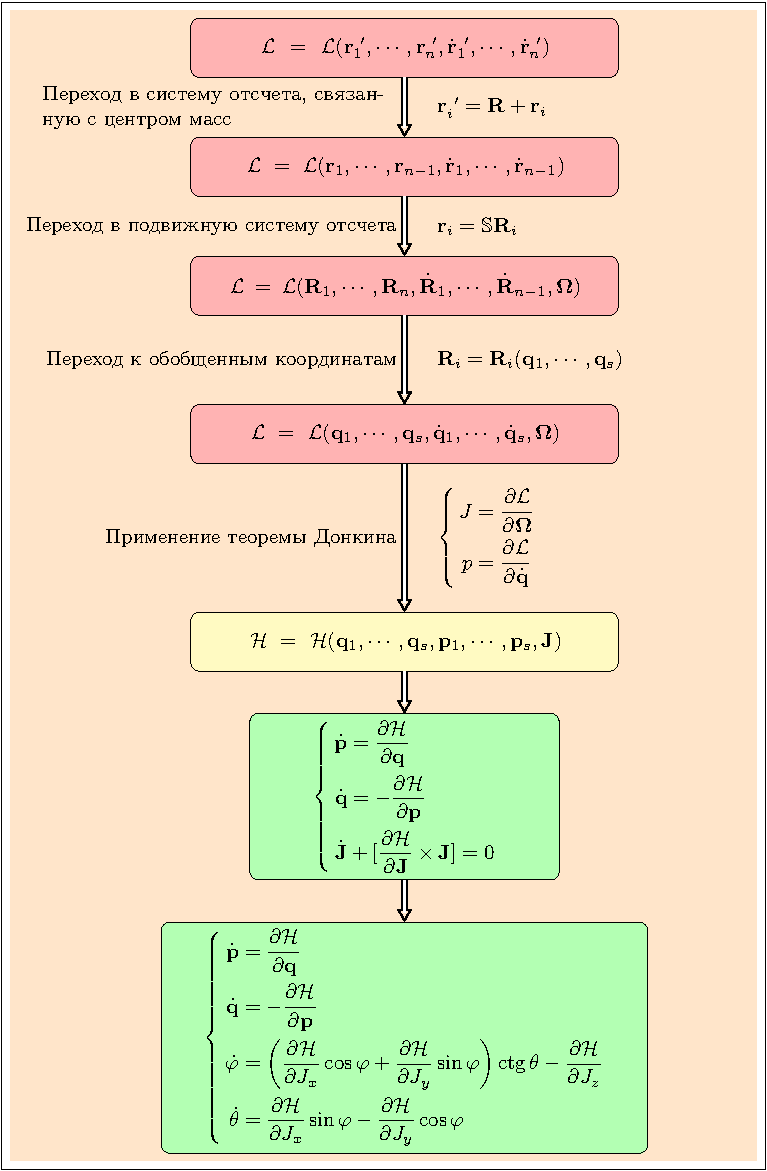
\includegraphics[width=0.85\linewidth]{pictures/flowchart.pdf}
        \end{tikzfigure}
   
   Первым шагом является получение лагранжиана системы в лабораторной системе координат. Стандартная процедура выделения центра масс позволяет сократить количество переменных. Переход от лабораторной системы отсчета к подвижной системе может быть осуществлен при помощи трех последовательных поворотов на углы Эйлера. 
    } 

    \column{0.25}
      \block[titleoffsety=1cm, bodyoffsety=1cm]{}{
       Применяя теорему Донкина, переходим к гамильтониану системы в подвижной системе отсчета. \\
        Полной системой динамических уравнений называют совокупность $2s$ уравнений Гамильтона и двух обобщенных уравнений Эйлера, где $s$ -- количество внутренних степеней свободы. Углы $\theta$, $\varphi$ описывают двумерное подпространство вращательной задачи в $(2s+2)$-мерном фазовом пространстве колебательно-вращательной задачи.}
    
    \block[titleoffsety=1cm, bodyoffsety=1cm]{Модельные системы}{
        \vspace*{-0.75cm}
        \begin{tikzfigure}
            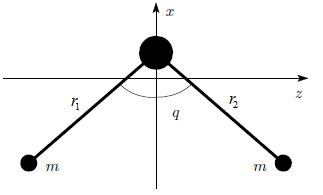
\includegraphics[width=0.75 \linewidth]{pictures/model.png}
        \end{tikzfigure}
        \vspace*{-0.5cm}

    В качестве первой системы была рассмотрена простейшая модель симметричной трехатомной молекулы $H_2X$. В первом приближении расстояние между легкими атомами и центральным атомом положим фиксированным. Таким образом, колебательная динамика молекулярной системы сводится к колебанию деформационного типа. В качестве потенциала, описывающего деформационное колебание, был взят потенциал Пешля-Теллера.
    \vverh
    \begin{gather}
        \mathcal{H} = \frac{1}{2 I_0} \left( \frac{J_x^2}{1 - \sin q} + \frac{J_y^2}{2} + \frac{J_z^2}{1 + \sin q} \right) + \frac{p^2}{I_0} + V, \quad I_0 = m r_0^2 \\
        V = \frac{1}{2 I_0} \left( \frac{V_{-}}{1 - \cos q} + \frac{V_{+}}{1 + \cos q} \right), \quad V_\pm = \frac{1}{4} I_0^2 \omega_0^2 \left( 1 \pm \cos q_0 \right) ^2 \notag
    \end{gather}

    Вторая модель представляет собой полноразмерную модель трехатомного гидрида, претерпевающего два валентных и деформационное колебания. Для описания валетного колебания использовался гармонический потенциал и реалистический потенциал Морзе.  
    \vverh
    \begin{gather}
        \mathcal{H} = \frac{1}{2I_0} \left( \frac{J_x^2}{1 - \cos q} + \frac{J_y^2}{2} + \frac{J_z^2}{1 + \cos q} + 2 \frac{r_1^2 - r_2^2}{r_1^2 + r_2^2} \frac{J_x J_z}{\sin q} \right) + \notag \\
        + \frac{r_1^2 - r_2^2}{2 m r_1^2 r_2^2} J_y p + \frac{p_1^2}{2m} + \frac{p_2^2}{2m} + \frac{p^2}{I_0} + U(r_1, r_2, q), \quad I_0 = \frac{2 m r_1^2 r_2^2}{r_1^2 + r_2^2} 
    \end{gather}
    }

    \block[titleoffsety=1.5cm,bodyoffsety=1.5cm]{Концепция поверхности вращательной энергии}{
        Поверхность вращательной энергии представляет собой двумерную поверхность. Величина вращательной энергии откладывается в направлении вектора углового момента относительно молекулярно-фиксированной системы координат (при фиксированном $J$). Концепция ПВЭ позволяет описать вращательную динамику молекулярной системы с точки зрения модели "мягкого тела".  
    \vverh
    \vverh
    \begin{gather}
        \left\{
        \begin{aligned}
            \left( \frac{\partial \mathcal{H}}{\partial \mathbf{q}} \right)_{\substack{\mathbf{q} = \mathbf{q}_e \\ \mathbf{p} = \mathbf{p}_e}} = \vec{0} \\
            \left( \frac{\partial \mathcal{H}}{\partial \mathbf{p}} \right)_{\substack{\mathbf{q} = \mathbf{q}_e \\ \mathbf{p} = \mathbf{p}_e}} = \vec{0}
        \end{aligned}
        \right. 
    \end{gather}
    
    }

    \column{0.25}
    
    \block[titleoffsety=1cm,bodyoffsety=1cm]{}{

        При фиксированном $\mathbf{J}$ внутренние координаты находят некоторое новое равновесное состояние ($\displaystyle \mathbf{q}_e$, система $(3)$), определяемое величиной центробежных сил. В рамках данного описания внутримолекулярные колебания отсутствуют и молекула вращается вокруг фиксированной в пространстве оси. 

    \begin{tikzfigure}[\large Перестройка поверхности вращательной энергии $H_2O$ при увеличении $J$: $J=10,30,50$.]
        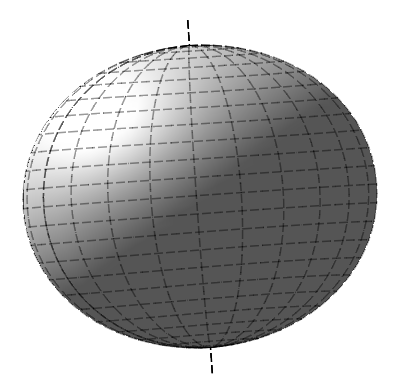
\includegraphics[width=0.45\linewidth]{pictures/Rigid_RES_10.png}
        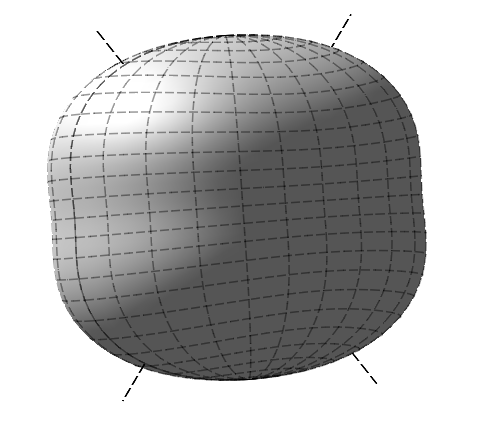
\includegraphics[width=0.45\linewidth]{pictures/Rigid_RES_30.png} \\
        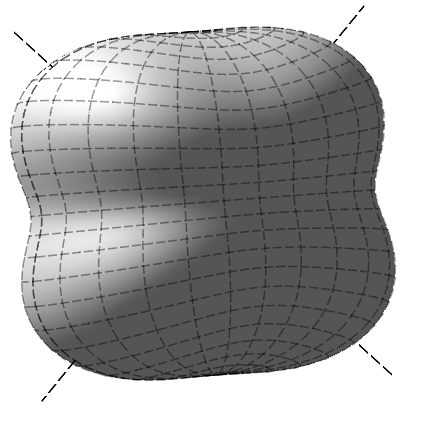
\includegraphics[width=0.45\linewidth]{pictures/Rigid_RES_50.png}
    \end{tikzfigure}

    При малых значениях момента ПВЭ имеет две устойчивые оси вращения $Oz$, $Oy$ и одну неустойчивую ось, проходящую через пару симметричных седловых точек. Таким образом, на ПВЭ имеется два типа прецессионных движений вектора $\mathbf{J}$. Анализ стационарных точек показывает, что перестройка ПВЭ наступает при достижении критического значения $J$: $J_{cr.} = \displaystyle \sqrt{V_{-} - V_{+}} = I_0 \, \omega_0 \displaystyle \sqrt{|\cos q_0|}$. При перестройке поверхности две точки максимума теряют свою устойчивость и становятся седловыми точками, одновременно с этим возникают четыре новых точки максимума с координатами $ (\theta_e, 0), (\theta_e, \pi), (\pi - \theta_e, 0), (\pi - \theta_e, \pi)$, где $\theta_e = \displaystyle \frac{1}{2} \arcsin \left( \displaystyle \frac{V_{-} - V_{+}}{J^2} \right)$.
}

\block[titleoffsety=1.5cm,bodyoffsety=1.75cm]{Фазовые траектории}{
C ростом полной колебательно-вращательной энергии влияние колебательной подсистемы на вращение молекулы не может быть учтено в рамках концепции ПВЭ. Система динамических уравнений, полученная для гамильтониана $(1)$, выглядит следующим образом: 
\vspace*{-0.3cm}
\begin{gather}
\left\{
\begin{aligned}
\dot{\Phi} &= \left( \frac{J \cos \Phi \sin \Theta}{I_0 ( 1 - \cos q)} \cos \Phi + \frac{J \sin \Phi \sin \Theta}{2I_0} \sin \Phi \right) \ctg \Theta - \frac{J \cos \Theta}{I_0 (1 + \cos q)} \\
\dot{\Theta} &= \frac{J \cos \Phi \sin \Theta}{I_0 (1 - \cos q)} \sin \Phi - \frac{J \sin \Phi \sin \Theta}{2I_0} \cos \Phi \\
\dot{q} &= 2	\frac{p}{I_0} \\
    \dot{p} &= - \frac{\sin q}{2I_0} \left( \frac{J^2 \cos^2 \Theta}{(1 + \cos q)^2} - \frac{J \cos^2 \Phi \sin^2 \Theta}{(1 - \cos q)^2} \right) - \\ & \quad \quad \quad \quad \quad \quad \quad \quad \quad \quad \quad  - \frac{1}{2I_0} \left( \frac{V_{+} \sin q}{(1 + \cos q)^2} - \frac{V_{-} \sin q}{(1 - \cos q)^2} \right)
\end{aligned}
\right. \notag
\end{gather}    
}

\column{0.25}
\block[titleoffsety=1cm,bodyoffsety=1cm]{}{

Фазовые траектории вращательной подзадачи описывают динамику конца вектора $\mathbf{J}$. Ниже представлена серия фазовых траекторий основного колебательного состояния с разными значениями $J$.

    \vspace*{-0.45cm}
    \begin{tikzfigure}[\large Динамика вектора углового момента модельной системы с деформационной степенью свободы в основном колебательном состоянии. Начальные параметры системы:
	\textbf{первый ряд} : $\Phi_0 = 0$, $\Theta_0 = 0.15$, $J = 10, \, 15, \, 20$ (\textit{до бифуркации});
	\textbf{второй ряд} : $\Phi_0 = 0$, $\Theta_0 = 0.15$, $J = 21, \, 22$ (\textit{после бифуркации});]
        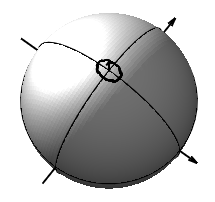
\includegraphics[width=0.30\linewidth]{pictures/plot_J=10n=0.png}
        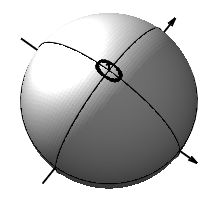
\includegraphics[width=0.30\linewidth]{pictures/plot_J=15n=0.png}
        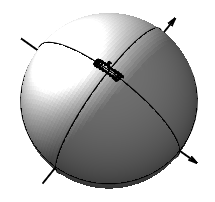
\includegraphics[width=0.30\linewidth]{pictures/plot_J=20n=0.png}\\
        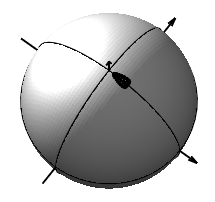
\includegraphics[width=0.30\linewidth]{pictures/plot_J=21n=0.png}
        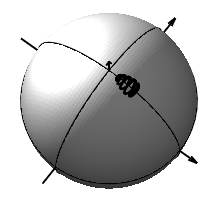
\includegraphics[width=0.30\linewidth]{pictures/plot_J=22n=0.png}
    \end{tikzfigure}

    \vspace*{-1.0cm}
    \begin{tikzfigure}[\large Динамика вектора углового момента полной модельной системы с валентным потенциалом гармонического типа в основном колебательном состоянии ${n = 0, n_1 = 0, n_2 = 0}$. Модуль вектора углового момента: $J = 10, \, 15, \, 20, \, 22, \, 24, \, 26$.]
        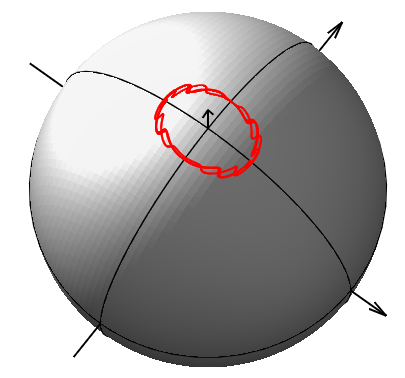
\includegraphics[width=0.30\linewidth]{pictures/HarmGroundState00/plot_J=10.png}
        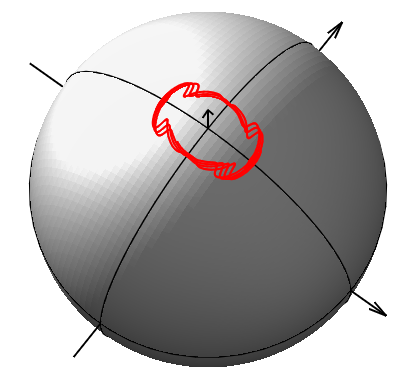
\includegraphics[width=0.30\linewidth]{pictures/HarmGroundState00/plot_J=15.png}
        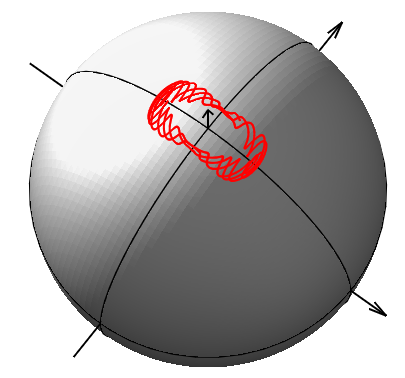
\includegraphics[width=0.30\linewidth]{pictures/HarmGroundState00/plot_J=20.png} \\
        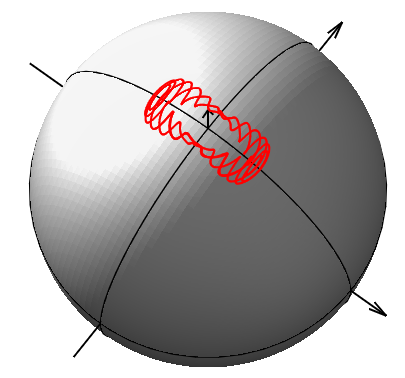
\includegraphics[width=0.30\linewidth]{pictures/HarmGroundState00/plot_J=22.png}
        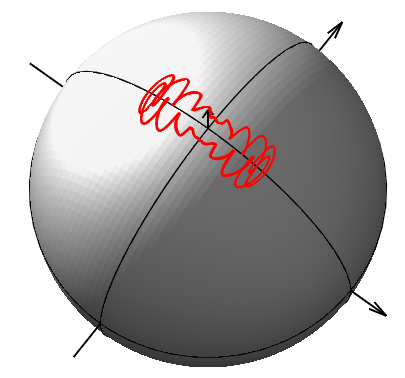
\includegraphics[width=0.30\linewidth]{pictures/HarmGroundState00/plot_J=24.png}
        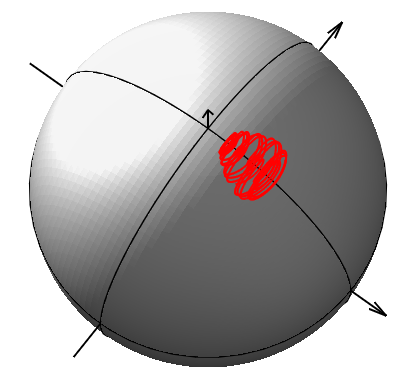
\includegraphics[width=0.30\linewidth]{pictures/HarmGroundState00/plot_J=26.png}
    \end{tikzfigure}
    
    \vspace*{-0.5cm}
При малых значениях момента фазовая траектория имеет достаточно сложный профиль, значительно отличающийся от эллипитического прецессионого профиля, наблюдаемого для модели с единственной деформационной степенью свободы. С ростом $J$ выделяются циклические структуры в окрестности тех положений, где ожидается возникновение новых устойчивых осей вращения, однако лишь при достижении значительно более высокого значения момента ($J=26$) происходит локализация траектории вокруг новой устойчивой оси.

}

\block[titleoffsety=1.5cm,bodyoffsety=2.5cm]{Выводы}{
    \begin{itemize}
        \item Описан метод получения точного колебательно-вращательного гамильтониана
        \item Получены гамильтонианы для одномерной и полномерной моделей трехатомного гидрида
        \item Описана бифуркация в рамках концепции поверхности вращательной энергии
        \item Получены решения полной системы динамических уравнений и описана бифуркация в фазовом пространстве вращательных траекторий
    \end{itemize}

}

\end{columns}

\end{document}
